% Monografia para Projeto de Fim de Curso - Exemplo no LaTeX
%-----------------------------------------------------------


%---------------Inicializa��o de pacotes--------------------

\documentclass[12pt,a4paper,notitlepage,twoside]{book}
\usepackage{times}

\usepackage{graphicx}
\usepackage[latin1]{inputenc}
\usepackage[brazil]{babel}
\usepackage[T1]{fontenc}
\usepackage{amsmath}
\usepackage{amsthm,amsfonts}
\usepackage{color}
\usepackage[colorlinks]{hyperref}
\usepackage{abntex2abrev}


\usepackage[a4paper,top=30mm,bottom=30mm,inner=30mm,outer=25mm,headheight=7mm,headsep=6mm,footskip=7mm]{geometry}
%\usepackage{epsfig}
%\usepackage{latexsym}
%\usepackage{float}
%\usepackage{quotes}
%\pagestyle {plain}

\makeindex

\def\baselinestretch{1.0}

%---------------In�cio do documento-------------------------

\begin{document}

\begin{titlepage}
\begin{center}
{\large Universidade Federal de Minas Gerais\\
Escola de Engenharia \\
Curso de Gradua��o em Engenharia El�trica\\}

\vspace{6cm}
{\bf\Large Separa��o de Fontes de �udio\vspace{0.2cm}
}
%Segunda Linha do T�tulo, se Houver}
\vspace{4cm}

%\hspace{0.3\textwidth} \parbox{0.65\textwidth}
{\large Kayke Renan Campos Silva}
\vspace{2cm}  
   
\vspace{2cm}          
%\hspace{0.3\textwidth} 
{\large Orientador: Prof. Adriano Vilela Barbosa}\\
%{\large Supervisor: Eng. Cicrano}

\vfill
%\hspace{0.3\textwidth} 
{\large Belo Horizonte, Dezembro de 2023 }
\end{center}

\end{titlepage}

\newpage
\clearpage
\thispagestyle{empty}


\begin{titlepage}

\centering
\textbf{Monografia}\\
\vspace{2cm}
\centering
\textbf{Separa��o de Fontes de �udio}\\
\vspace{5cm} 

\parbox{1.0\textwidth} 
{\large 
Monografia submetida � banca examinadora
designada pelo Colegiado Did�tico do Curso de
Gradua��o em Engenharia El�trica da Universidade Federal de Minas
Gerais, como parte dos requisitos para aprova��o na
disciplina Trabalho de Conclus�o de Curso.}

\vspace{7cm} 
\centering
Belo Horizonte, Dezembro de 2023

\end{titlepage}


\pagenumbering{roman}
\addcontentsline{toc}{chapter}{Resumo}

\begin{center}
\huge{{\bf Resumo}}
\vspace{2cm}
\end{center}

No Resumo, normalmente em uma �nica p�gina, voc� escreve um par�grafo para cada um dos seguintes itens: objetivos do projeto e descri��o sucinta do local onde ele foi desenvolvido; 
metodologia utilizada; e resultados alcan�ados.
 
\begin{sloppypar}
Este novo par�grafo serve para mostrar que ao pular uma ou mais linhas no texto do arquivo .tex, o \TeX\ entende que voc� est� iniciando outro par�grafo. O comando sloppypar for�a o texto a n�o ultrapassar as margens. S� deve ser usado se este problema ocorrer.
\end{sloppypar}

 
\clearpage
\thispagestyle{empty}
\cleardoublepage


\addcontentsline{toc}{chapter}{Agradecimentos}

\begin{center}
\huge{{\bf Agradecimentos}}
\vspace{4cm}
\end{center}

Aqui vai o texto dos agradecimentos.
 
\clearpage
\thispagestyle{empty}
\cleardoublepage
\tableofcontents
%\markboth{Conte�do}{Conte�do}

\clearpage
%\thispagestyle{empty}
%\cleardoublepage

% Normalmente, este arquivo s� cont�m isto.
\listoffigures
\addcontentsline{toc}{chapter}{Lista de Figuras}
%\markboth{Lista de Figuras}{Lista de Figuras}

\clearpage
%\thispagestyle{empty}
%\cleardoublepage

% Normalmente, este arquivo s� cont�m isto.
\listoftables
\addcontentsline{toc}{chapter}{Lista de Tabelas}
%\markboth{Lista de Tabelas}{Lista de Tabelas}

\clearpage
%\thispagestyle{empty}
%\cleardoublepage

% Normalmente, este arquivo s� cont�m isto.

\pagenumbering{arabic}
\setcounter{page}{1}
\chapter{Introdu��o}
%\markboth{\thechapter ~~~ Introdu��o}{}
%\label{intro}

A separa��o de fontes de �udio, em ingl�s \textit{Audio Source Separation (ASS)}, consiste no problema de simular a capacidade do sistema auditivo humano de extrair uma fonte de �udio de interesse dentre outras fontes misturadas e ru�dos. Este problema � conhecido na literatura como o "efeito da festa de coquetel" (\textit{the cocktail party effect}) ou "escuta seletiva" \cite{web:cocktail}, descrito como um ambiente de festa com a presen�a de diversas pessoas conversando, possivelmente com m�sica e outros ru�dos onde um indiv�duo � capaz de ignorar e suprimir as diversas fontes sonoras enquanto foca e extrai apenas aquela(s) que o interessa, seja uma conversa, m�sica, instrumento(s), etc.


\section{Motiva��o e Justificativa}
\markright{\thesection ~~~ Motiva��o}
%\label{motiva}

A separa��o de fontes de �udio (ASS) � um caso especial do problema geral de separa��o de fontes na �rea de processamento de sinais que decorre do fato de que os sinais no mundo real geralmente v�m misturados com outros sinais e ru�dos, especialmente no dom�nio eletromagn�tico pelo fen�meno de acoplamento que ocorre quando os sinais compartilham um mesmo canal de transmiss�o e/ou ambiente de gera��o, por exemplo os sinais biol�gicos captados por eletrodos, ondas eletromagn�ticas em telecomunica��es, etc.

Quando os diferentes sinais possuem bandas espectrais distintas, o problema de separa��o pode ser solucionado atrav�s da filtragem, como ocorre nos sistemas de telecomunica��es atrav�s da modula��o e demodula��o, mas quando os espectros se sobrep�em, a solu��o � mais dif�cil por se tratar de um problema inverso \cite{web:inverse}. Neste tipo de problema busca-se, a partir de observa��es de um fen�meno em um determinado dom�nio, inferir as causas ou os melhores modelos, geralmente em um outro dom�nio, que explicam e/ou aproximam os dados observados. Como exemplo, pode-se citar a descoberta de Netuno a partir de medi��es que indicavam desvios da previs�o te�rica da �rbita de Urano.

A separa��o de fontes � um problema ainda em aberto e portanto diversas abordagens para abord�-lo foram e t�m sido propostas, combinando heur�sticas e diferentes m�todos computacionais, assim como informa��es sobre os sinais e o processo de mistura quando poss�vel. O interesse no problema de separa��o de fontes se justifica pelo fato de que os resultados podem ser aplicados a diversos outros problemas, como a separa��o de instrumentos para remixagem de m�sicas antigas que dispunham de poucos canais no processo de grava��o, extra��o de voz e outras informa��es em grava��es de �udio para uso em per�cia criminal, separa��o de sinais biol�gicos em exames e pesquisas, cancelamento de ru�dos em fones de ouvidos e em microfones visando melhorar a qualidade das comunica��es, dentre outras aplica��es.

Este trabalho ter� como foco o caso especial de separa��o de instrumentos musicais em grava��es, tendo como inspira��o os recentes resultados obtidos com a re-mixagem do disco \textit{Revolver} da banda \textit{The Beatles}. Na �poca da grava��o do disco, apenas 4 canais de �udio estavam dispon�veis, de forma que diversos instrumentos tiveram de ser misturados em cada trilha, tornando a separa��o dos instrumentos para re-mixagem um problema sem resultados satisfat�rios atrav�s das t�cnicas cl�ssicas, tornando-se poss�vel apenas recentemente com a aplica��o de sistemas de redes neurais profundas, como declarado pelo produtor Giles Martins, respons�vel pela re-mixagem da discografia da banda \cite{web:giles}.


\section{Objetivos do Projeto}
\markright{\thesection ~~~ Objetivos}
%label{objetivos}

%Tendo em vista o exposto acima, este projeto tem por objetivos:

%\begin{itemize}
%\item[a.] Item 1;
%\item[b.] Item 2;
%\item Etc.
%\end{itemize}

O trabalho consiste em implementar e comparar os resultados da separa��o de 4 instrumentos (bateria/instrumentos per
cursivos, vocais, guitarras e baixo) utilizando duas abordagens, uma mais cl�ssica com o m�todo computacional de fatora��o de matrizes n�o-negativas, como descrito no estudo \cite{tygel} e outra abordagem mais recente (informar sobre os per�odos de tempo em que cada uma foi proposta e estudada) utilizando aprendizado de m�quina a partir de redes neurais profundas com aux�lio da biblioteca em Python Open-Unmix [5]. A escolha dos instrumentos se deu pela facilidade de encontr�-los em diversas m�sicas de g�neros diferentes, al�m do fato de separar em instrumentos que possuem afina��o (vocais, guitarras e baixo) e que n�o possuem afina��o (bateria e instrumentos percussivos)

A compara��o dos resultados se dar� a partir de um estudo com um n�mero de pessoas ainda a ser definido, em que inicialmente ser� apresentada uma grava��o musical com a mistura dos instrumentos e em seguida, de forma randomizada sem que o participante saiba qual m�todo est� sendo apresentado, para cada instrumento separado perguntar se alguma dos m�todos teve um desempenho melhor do que o outro ou se apresentam a mesma qualidade. 

Ap�s esta etapa de sele��o do melhor m�todo para cada instrumento, ser� apresentado novamente para cada participante aquelas trilhas de cada instrumento que foram escolhidas por este como as melhores, sendo que no caso de empate ser� escolhido um dos m�todos de forma aleat�ria, e em seguida ser� pedido para ordenar a qualidade de separa��o de cada instrumento do melhor para o pior ou se apresentam a mesma qualidade. A partir destes resultados, ser� poss�vel decidir se algum m�todo teve um desempenho estatisticamente melhor do que o outro e se dentro de cada m�todo a qualidade de separa��o para cada instrumento varia ou n�o.

A op��o pelo estudo com participantes se d� pelo fato do ser humano ser considerado o padr�o ouro com rela��o � capacidade de separa��o de fontes de �udio e por n�o ter atualmente um modelo psicoac�stico que consiga reproduzir de forma objetiva a habilidade humana. A op��o pela compara��o qualitativa entre os m�todos vem da dificuldade de se atribuir n�meros absolutos para a qualidade da separa��o que demandam m�tricas e m�todos estat�sticos mais complexos, portanto optou-se pela simplicidade al�m do fato de n�o exigir dos participantes alguma forma de conhecimento pr�vio da tarefa de separa��o dos sinais e a consequente medi��o da qualidade, bastando apenas sua percep��o.



%\section{Local de Realiza��o}
%\markright{\thesection ~~~ A Empresa}
%\label{empresa}

%Vale � pena descrever a empresa onde o TCC foi desenvolvido. Veja o exemplo abaixo.

%O trabalho de conclus�o de curso foi desenvolvido na empresa ..., no Departamento de ..., respons�vel por toda a implementa��o do sistema de ...

%A empresa realiza projetos de pesquisa e desenvolvimento, consultoria e treinamento nas �reas de ...

%A ... foi criada em ...  

%A empresa � divida em tr�s departamentos: (o arquivo Introducao.tex mostra como criar a lista abaixo) 

%\begin{itemize}
%\item Departamento de ... 
%\item Departamento de ...
%\item Departamento de ...
%\end{itemize}

%Este projeto foi desenvolvido no Departamento de ..., que � o respons�vel por ...

%Os demais Departamentos englobam as fun��es de ...

%Todos os departamentos trabalham em conjunto. O Departamento de ..., por exemplo, precisa manter um grande v�nculo com o Departamento de ... Isso ocorre porque todas as especifica��es de hardware e sistemas influenciam a forma de implementa��o de servi�os, organiza��o de tabelas e recursos dispon�veis.




%\section{Estrutura da Monografia}
%\markright{\thesection ~~~ Organiza��o do Trabalho}
%\label{organiza}

%O trabalho est� dividido em quatro cap�tulos. Este cap�tulo apresentou uma introdu��o ao projeto a ser descrito nesta monografia e a empresa onde o trabalho foi realizado. O Cap�tulo 2 descreve os princ�pios b�sicos de um sistema ... (sistema onde se insere o trabalho) e abrange todos os conceitos necess�rios para um melhor entendimento do projeto. O Cap�tulo 3 aborda a metodologia de desenvolvimento, seguida pela implementa��o dos .... No Cap�tulo 4 tem-se a conclus�o da  monografia e algumas sugest�es e dificuldades encontradas na realiza��o do projeto.


\clearpage
%\chapter{Descri��o do Processo}

Se desejar, uma vis�o geral do Cap�tulo pode ser colocada antes da primeira Se��o. Este � o cap�tulo de descri��o do processo e formula��o do problema. Tendo em vista que se trata de uma monografia de engenharia de controle e automa��o, em muitos casos, � fundamental a apresenta��o dos sensores e atuadores do processo.


\section{Processo de Fazer Alguma Coisa}
\markright{\thesection ~~~ Hist�rico}
\label{hist}

...


\section{Instrumenta��o do Processo}
\markright{\thesection ~~~ O Telefone}
\label{telefone}



Continua ...


\section{Resumo do Cap�tulo}

N�o termine de forma abrupta.



\clearpage

\chapter{Metodologia e Revis�o Bibliogr�fica}

Neste cap�tulo, voc� deve apresentar uma breve revis�o bibliogr�fica sobre as t�cnicas utilizadas para solu��o do problema.


Ao longo do tempo, diversas t�cnicas e abordagens foram desenvolvidas e aplicadas ao problema de ASS, levando a diferentes linhas de pesquisa em que todas t�m em comum a aplica��o em maior ou menor grau de conceitos e ferramentas de processamento de sinais, modelagem de fontes de �udio como fonte-filtro, �lgebra linear, probabilidade e estat�stica \cite{rafii18}. Al�m disso, sinais de �udio multicanais (como �udio est�reo, surround 5.1, surround 7.1) demandam t�cnicas diferentes daquelas utilizadas em sinais que possuem apenas um canal (�udio mono), contribuindo ainda mais para a diversidade de linhas de pesquisa.

\section{Blind Source Separation e An�lise de Componentes Independentes}
Historicamente, as primeiras abordagens para tratar o problema partiram de simplifica��es da teoria de sinais e sistemas din�micos lineares em que a partir de um n�mero conhecido F de fontes e um n�mero conhecido S de sensores (microfones), os sinais captados por cada microfone no dom�nio do tempo poderiam ser representados a partir da convolu��o entre o sinal de cada fonte e a resposta ao impulso do sistema composto pela agrega��o dos efeitos de propaga��o e interfer�ncia agindo entre cada fonte e o sinal captado pelo sensor (como a reverbera��o do ambiente de grava��o, interfer�ncias de outras fontes, filtros dos circuitos eletr�nicos dos sensores, etc.). Como pode-se notar, ainda que simplifica��es na forma da premissa de o n�mero de fontes ser conhecido e o fato deste tipo de modelo de respostas ao impulso considerar que as fontes s�o pontuais e estacion�rias [7], a identifica��o e modelagem do sistema din�mico atrav�s das respostas ao impulso n�o � uma tarefa trivial e geralmente sequer poss�vel, portanto, foram necess�rias simplifica��es adicionais deste problema como a considera��o da escassez de informa��o sobre as fontes e sobre o processo de mistura no que � conhecido na literatura como Blind Source Separation (BSS) [8] e [9], na qual a t�cnica de An�lise de Componentes Independentes (Independent Component Analysis - ICA) � uma das mais exploradas at� hoje. 

A ICA faz uma s�rie de suposi��es simplificadoras, dentre elas que as fontes s�o estatisticamente independentes, que a mistura pode ser modelada como uma simples combina��o linear dos sinais da fonte (ou seja, a mistura � apenas instant�nea e efeitos de convolu��o n�o s�o modelados), al�m de que a solu��o do sistema linear formado pode ser obtida apenas quando h� um n�mero de microfones igual ou maior do que o n�mero de fontes (S >= F). A formaliza��o matem�tica da ICA assim como melhorias do m�todo visando resolver as limita��es de n�mero de fontes, efeitos de convolu��o e n�o-linearidades do processo de mistura s�o exploradas em [10] dado que os sinais de �udio de forma geral n�o atendem �s restri��es impostas pela t�cnica, por exemplo o fato da maioria ser no formato mono ou est�reo e possuir mais do que duas fontes sonoras.

\section{M�scaras Espectrais}
Outra abordagem derivada diretamente da teoria de processamento de sinais consiste na filtragem do sinal misturado, isto �, realizar uma esp�cie de equaliza��o na mistura atenuando ou amplificando determinadas frequ�ncias assumindo que diferentes fontes apresentam caracter�sticas e regi�es espectrais diferentes, por�m, como o sinal de �udio muda ao longo do tempo, � necess�rio que esta equaliza��o tamb�m mude de forma correspondente, portanto, de forma a obter este efeito, utilizam-se m�scaras espectrais que consistem em filtros cujas caracter�sticas s�o variantes no tempo [11], portanto, as m�scaras espectrais operam tanto no dom�nio da frequ�ncia quanto no dom�nio do tempo simultaneamente, logo, sua aplica��o se d� numa representa��o Tempo-Frequ�ncia do sinal como o espectrograma do sinal misturado. Uma breve explica��o do espectrograma � feita no cap�tulo de fundamentos te�ricos.

--------------- 

\textbf{Trecho do cap�tulo de fundamentos te�ricos explicando o espectrograma}

O espectrograma � uma representa��o de como o espectro de frequ�ncias do sinal varia ao longo do tempo obtido atrav�s da transformada de Fourier (TF) de tempo curto (STFT), onde definem-se intervalos de tempo (janelas/bins) nos quais ser�o realizados a TF de forma sucessiva ao longo da dura��o do sinal. O espectrograma � obtido a partir da magnitude da TF para cada intervalo de tempo, como ilustrado na figura [REF.], onde o eixo vertical corresponde �s frequ�ncias, o eixo horizontal ao tempo e a cor de cada ponto a intensidade/magnitude da TF naquela frequ�ncia naquela janela de tempo.

------------------

Existem diversas t�cnicas para obter m�scaras espectrais de acordo com as caracter�sticas do sinal (como o n�mero de canais) e premissas sobre as fontes misturadas (como o n�mero de fontes, a distribui��o espectral de cada uma, etc.) e a separa��o � obtida atrav�s da multiplica��o matricial da m�scara pela representa��o tempo-frequ�ncia do sinal.
Para o caso em que h� apenas um canal, a m�scara espectral � geralmente representada como uma matriz de valores reais entre 0 e 1. Al�m disso, elas podem ser classificadas de acordo com os valores que podem assumir, como as m�scaras bin�rias que s�o restritas apenas aos valores 0 e 1 (i.e., de forma discreta) e que s�o aplicadas em problemas de separa��o de fala [12], enquanto as m�scaras que podem assumir qualquer valor real entre 0 e 1 s�o classificadas como soft-masks ou ratio-masks e apresentam desempenho superior �s m�scaras bin�rias como demonstrado nos estudos [13] e [14] em que a separa��o obtida apresenta uma melhor rela��o sinal-ru�do (SNR). J� quando o sinal � multicanal, dificuldades adicionais como a diferen�a de tempo entre os sinais da mesma fonte em cada canal devem ser levadas em conta e como consequ�ncia as m�scaras espectrais passam a ser representadas como matrizes de valores complexos de forma a modelar a diferen�a de fase entre os sinais.

\section{Modelagem Fonte-Filtro}
Outra abordagem envolve a modelagem das diferentes fontes de �udio a partir do modelo fonte-filtro constitu�do por um sinal de excita��o (a fonte) que � alterado por um filtro que representa alguma caracter�stica do meio ou instrumento. A altera��o do sinal pelo filtro se d� pela mudan�a do envelope espectral do sinal. Esta abordagem � muito utilizada na modelagem de voz como em [15], onde a fonte do sinal de excita��o corresponde aos pulsos glotais gerados pelas cordas vocais e o filtro corresponde ao trato vocal.

Outra possibilidade � a modelagem tanto de melodias cantadas por vozes quanto de instrumentos afinados dado que em teoria musical as notas s�o determinadas por frequ�ncias espec�ficas (chamadas de frequ�ncias fundamentais) e o timbre dos instrumentos � derivado do envelope espectral dos harm�nicos que s�o m�ltiplos inteiros da frequ�ncia fundamental, logo, pode-se modelar a fonte como o sinal senoidal puro com a frequ�ncia fundamental e o timbre atrav�s do filtro. Al�m disso, esta modelagem � facilitada dado que geralmente apenas um conjunto reduzido de notas ocorrem em cada m�sica por causa de conceitos de teoria musical como escala, tom, campo harm�nico, etc.

O modelo fonte-filtro e as considera��es sobre a caracter�stica harm�nica de instrumentos e melodias cantadas necessitam de m�todos de identifica��o da frequ�ncia fundamental assim como a sua correspondente varia��o ao longo do tempo para extra��o das melodias. Estes m�todos em conjunto com o modelo fonte-filtro foram explorados em trabalhos como em [16] onde ap�s realizar a identifica��o das frequ�ncias fundamentais ao longo da melodia atrav�s da STFT, realizou-se a sintetiza��o das fontes atrav�s do modelo fonte-filtro de cada uma. Abordagem similar foi utilizada no trabalho [17] de forma a separar sinais musicais de voz acompanhada de piano. Por�m os resultados obtidos pela sintetiza��o a partir do modelo fonte-filtro e da harmonicidade sofrem do problema de soarem artificiais pela caracter�stica metalizada, como discutido em [6], decorrente das diferen�as entre os sinais de excita��o estimados para as fontes e os sinais reais, o que exp�e a sensibilidade destes m�todos � qualidade do modelo fonte-filtro e � qualidade de extra��o da melodia o que impede a aplica��o em grava��es que fogem das condi��es ideais que o m�todo exige. Al�m disso, nem todos instrumentos podem ser modelados como harm�nicos, como � o caso de instrumentos percussivos, demandando portanto novas abordagens.

\section{Fatora��o e Co-Fatora��o de Matrizes N�o-Negativas}
De forma a atacar as limita��es dos m�todos harm�nicos com modelo fonte-filtro, outras abordagens passaram a considerar a natureza repetitiva de sinais musicais, como as repeti��es r�tmicas, as repeti��es de notas em escalas, as de acordes na progress�o harm�nica e as repeti��es de estruturas musicais como versos e refr�es presentes em m�sicas populares. Essas repeti��es podem ser modeladas como um conjunto de estruturas b�sicas (features) que aparecem e s�o combinadas em determinados momentos, no caso de sinais musicais isso corresponde a considerar que o espectrograma da mistura pode ser decomposto em poucos espectrogramas bases que s�o ativados e combinados ao longo do tempo, sendo este o fundamento do algoritmo de fatora��o de matrizes n�o-negativas (Non-negative Matrix Factorization - NMF) [18] em que uma matriz de valores n�o-negativos � decomposta como o produto entre outras duas matrizes tamb�m n�o negativas, sendo que o algoritmo � explicado com mais detalhes no cap�tulo de fundamentos te�ricos. O algoritmo de NMF foi aplicado em sinais musicais em [19] e [20], por�m como o algoritmo n�o garante unicidade de solu��es e por ser um caso especial de BSS, a interpreta��o da separa��o em instrumentos � prejudicada al�m do fato de que por ser um algoritmo de aproxima��o por ?low-rank?, ele n�o � adequado para vocais e instrumentos que apresentam menos repeti��es. De forma a atacar estes problemas, uma varia��o do algoritmo chamada de co-fatora��o de matrizes n�o-negativas visa realizar a fatora��o conjunta da matriz alvo (o espectrograma) e uma matriz contendo informa��o adicional como melodias, vocais e acompanhamento quando dispon�veis de forma que a fatora��o obtida apresenta componentes compartilhadas com as matrizes de informa��o, como mostrado pelos resultados em [21] e [22] para o caso de instrumentos percussivos e em [23] para vocais.

\section{Redes Neurais Artificias}
Atualmente as abordagens que t�m produzido resultados mais promissores e superiores aos m�todos j� explorados s�o aquelas baseadas em aprendizado de m�quina como redes neurais artificiais, dada a disponibilidade atual do grande volume de dados para treinamento. Como os m�todos discutidos acima s�o baseados sempre em alguma esp�cie de modelagem que exigem determinadas suposi��es que quando n�o satisfeitas produzem resultados insatisfat�rios, as abordagens por aprendizado de m�quina se destacam pela aus�ncia destas suposi��es, onde o modelo � obtido pelo treinamento a partir dos exemplos. A primeira aplica��o das redes neurais em ASS se deu em [24] com o emprego de redes neurais recorrentes (Recurrent Neural Networks - RNN). J� em [25], redes neurais convolucionais (Convolutional Neural Networks - CNN) foram utilizadas para extra��o de vocais. Em [26], os autores aplicaram redes neurais feedforward (Feedforward Neural Networks - FNN) para separa��o de instrumentos e re-mixagem de m�sicas de Jazz.

Os trabalhos mais recentes buscam associar redes neurais profundas com t�cnicas dos modelos descritos neste cap�tulo, aumentando assim o desempenho destes algoritmos, como em [27] que na sa�da de uma RNN foi inserida uma camada extra de uma m�scara espectral usada para gerar os espectros das fontes separadas e portanto o processo de aprendizado aproxima de forma indireta a m�scara espectral ideal que produz a melhor separa��o, onde os resultados obtidos superaram os algoritmos estado da arte em separa��o de voz.

Os problemas associados com o emprego de redes neurais s�o o custo computacional no treinamento dos algoritmos e a necessidade de uma grande base de dados para treinamento, al�m da dificuldade de interpreta��o dos milhares de par�metros dos modelos que estas redes geram [6].


\section{T�cnica 1}
\markright{\thesection ~~~ Metodologia}
\label{metodo}

Aqui voc� encontra um exemplo de inser��o de figura. Veja o arquivo DescricaoProjeto.tex para ver os comandos.
\begin{figure}[!htbp]
	\centering		
	\includegraphics[bb =0 0 264  221]{Resultados/Figuras/ciclodesenvolvimento.eps}
	\caption{figuara teste}
	\label{fig:ciclodesenvolvimento}
\end{figure}

A figura \ref{fig:ciclodesenvolvimento} tal aparece.

\begin{table}
	\centering
		\begin{tabular}{c|c}
			1 & 2 \\
			1 & 2 \\
			1 & 2 \\
			1 & 2 \\
			1 & 2 \\			
		\end{tabular}
\end{table}


\begin{figure}[htbp]
\centering
\includegraphics[scale=1.2]{Metodologia/Figuras/ciclodesenvolvimento.eps}
\caption{Ciclo de desenvolvimento de um projeto.}
\label{CicloDesenvolvimento1}
\end{figure}

Para referenciar a Figura \ref{CicloDesenvolvimento1}, veja arquivo .tex.

\begin{equation}\label{eq:forca}
	f=ma
\end{equation}

A equa��o \ref{eq:forca}
\section{T�cnica 2}
\markright{\thesection ~~~ Metodologia}
\label{metodo1a}

\section{Resumo do Cap�tulo}
\markright{\thesection ~~~ Metodologia}
\label{metodo1b}




\clearpage
\chapter{Resultados}

Para a execu��o do projeto, algumas etapas de desenvolvimento tiveram de ser seguidas: familiariza��o com o sistema, estudo dos m�dulos envolvidos, leitura dos requisitos, elabora��o de documento descrevendo todo o processo de implementa��o e relacionamento com os diversos m�dulos, implementa��o e testes.

\section{Atividades do Projeto}
\markright{\thesection ~~~ Metodologia}
\label{metodo3}

\section {Requisitos do Sistema}
\markright{\thesection ~~~ Requisitos}
\label{req}






\begin{figure}[htbp]
\centering
\includegraphics[scale=1.2]{Resultados/Figuras/ciclodesenvolvimento.eps}
\caption{Ciclo de desenvolvimento de um projeto}
\label{CicloDesenvolvimento}
\end{figure}

Para referenciar a Figura \ref{CicloDesenvolvimento}, veja arquivo .tex.



Aqui come�a uma sub-se��o.


\section{Desenvolvimeto e Implementa��o}

Aqui come�a outra se��o.

Para inserir a tabela abaixo, veja arquivo .tex.

\begin{table}
\centering
\begin{tabular}{|l|l|}\hline
		1.Uso do servi�o & Para o assinante rastrear uma chamada, ele dever� tirar\\ 
										 & o telefone do gancho, esperar pelo tom de discagem e ent�o \\
										 & discar o c�digo de acesso ao servi�o. \\ \hline
		2.Processamento  & Caso o assinante tenha acesso ao servi�o SRUC, ele dever�  \\			
		  do servi�o 		 & ouvir um an�ncio, ao discar o c�digo de acesso, explicando \\
									   & que o servi�o SRUC foi acessado. Dessa forma, se os dados \\
									   & a serem rastreados forem suficientes, o sistema dever� \\
									   & fornecer uma mensagem de confirma��o de \\
									   & servi�o realizado \\ \hline
		3. Ativa��o da   		& A ativa��o do servi�o somente ser� v�lida \\
			 �ltima chamada   & para a �ltima chamada recebida. \\ 
			 recebida				 	& \\ \hline
		4. Mais de uma   		& Se o assinante tentar ativar o servi�o para a mesma chamada \\
			 ativa��o para 	 	& ele dever� ouvir novamente o an�ncio de servi�o realizado, mas \\
			 a mesma chamada	& n�o ir� gravar os dados novamente \\ \hline
		5. N�mero privado 	& O sistema dever� mostrar o n�mero do assinante chamador \\
			 do assinante A  	& mesmo que este n�o possa ser mostrado. \\ \hline
		6. Chamadas  				& Para que o servi�o possa valer para chamadas intercentrais \\
			 intercentrais		& a central dever� utilizar a sinaliza��o SS7, e o n�mero do \\
												& assinante A ser� obtido pela mensagem IAM. \\ \hline
		7. Informa��es de 	& Um \textit{trace} do servi�o dever� possuir os seguintes itens:\\
			 um registro			& N�mero do assinante A \\
												& Hora da chamada recebida\\
												& Data da chamada recebida\\
												& N�mero do assinante B\\
												& Hora da solicita��o do servi�o\\
												& Data da solicita��o do servi�o\\
												& Dados sobre rota para chamadas intercentrais \\ \hline
		8. Tratamento para 	& Se um assinante discar o c�digo de acesso ao \\
		   assinante sem 		& servi�o, a central dever� fornecer tratamento padr�o \\
			 servi�o					& de acesso negado. \\ \hline
		9. Tipos de 				& A central deve permitir que o assinante com o servi�o \\
		   telefones				& possua tanto DTMF quando Dial Pulse \\ \hline
		10. Comandos do 		& O sistema supervis�rio conectado � central dever� \\
		    sistema 				& disponibilizar um  comando para que o operador possa  \\
		    supervis�rio		& descarregar o arquivo com os \textit{traces} das chamadas \\
		    								& para os diversos assinantes de uma central. \\
												& Um comando para visualizar os \textit{traces} tamb�m ser� necess�rio. \\ \hline
		\end{tabular}
	\caption{Requisitos do Servi�o SRUC}
	\label{tab:RequisitosDoServi�oSRUC}
\end{table}

Aqui voc� referencia a tabela: a Tabela \ref{tab:RequisitosDoServi�oSRUC} explicita os pontos mais relevantes na implementa��o do SRUC.

\section{Testes}

\section{Resumo do Cap�tulo}
\markright{\thesection ~~~ Metodologia}
\label{metodo4}
Esse cap�tulo pode ser dividido em duas partes $	f=ma $ blaba
 
\begin{gather}
	f=ma\\
	x=2\\
\end{gather}

\begin{align}
	f=ma\\
	x=2\\
\end{align}

\begin{eqnarray}
	f=ma\\
	x=2\nonumber\\
\end{eqnarray}


\clearpage
\chapter{Conclus�es}

\section{Considera��es Finais}

Aqui vai o texto da conclus�o.

\section{Propostas de Continuidade}


\clearpage


\addcontentsline{toc}{chapter}{Refer�ncias Bibliogr�ficas}
\bibliographystyle{unsrt}
\begin{small}
\bibliography{telefonia}
\end{small}

\end{document}

%---------------Fim do documento----------------------------